\documentclass{article}
\usepackage{stocktonmacros} % Personal macros, import package
\setlist[itemize]{noitemsep, topsep=0pt} % Must keep within the same document as \begin{document}

\begin{document}

%\maketitle
%%
%\newpage
%%
%\tableofcontents
%%%
%\newpage
%%%
%\import{Lectures/}{Partial Differential Equations - An Introduction}
%\import{Lectures/}{Heat, Wave Equation}
%\import{Lectures/}{Approximating Functions with Other Functions}
%\import{Lectures/}{Heat Equation}
%\import{Lectures/}{Wave Equation}
%\import{Lectures/}{Boundary Conditions}
%\import{Lectures/}{Laplace's Equation}
%\import{Lectures/}{Polar Coordinates}
%\import{Lectures/}{Complex Analysis, Fourier Transform}
%\import{Lectures/}{Transport Equation}
%\import{Lectures/}{Image Processing}
%\import{Lectures/}{Exam 2 Review}
\import{Lectures/}{Conservation Laws}
%______________________________________________________________________________%
\newpage
% Conservation Law?
\subsection{Traffic Flow}
\topic{April 11, 2022}
Conservation of Cars

Traffic in - Traffic out = Accumulated traffic

\begin{center}
  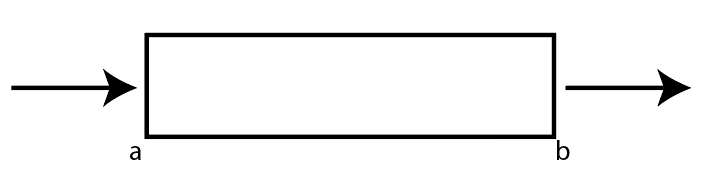
\includegraphics{Conservation Laws - Traffic Flow 1}
\end{center}

Let $\rho(x, t)$ be the density and $q(x, t)$ is the flux.
%
\begin{align}
  \frac{d}{dt} \int^b_a \rho(x, t)\ \text dx
  & = q(a, t) - q(b, t)\\
  & = -\int^b_a q_x (x, t)\ \text dx\\
  \int^b_a (\rho_t + q_x)\ \text dx & = 0\\
  \rho_t + q_x & = 0
\end{align}

Here, $u$ is car velocity:
%
\begin{align}
  q & = pu
\end{align}

Now,
%
\begin{align}
  \rho_t + [\rho u]_x & = 0
\end{align}

Both $\rho$ and $u$ are a function of $x$, therefore there is a product rule that comes into play.
%
\begin{align}
  \rho_t + [c(\rho)]\rho_x & = 0
\end{align}

We have yet to determine $c$. So far, this equation is similar to the Transport Equation, where we use $c$ to find the speed of the equation.

$c(\rho)$ will give the speed of the characteristic.

In general, the car velocity should be a decreasing function of $\rho$.

When $\rho = 0$, the car moves the fastest $= u_{\text{max}}$

When $\rho = \rho_{\text{max}} \Rightarrow u = 0$

The simplest relationship which satisfies these is:
%
\begin{align}
  u(\rho) & = u_{\text{max}}\left(1 - \frac{\rho}{\rho_{\text{max}}}\right)
\end{align}

This tells me,
%
\begin{align}
  q(\rho)
  & = u_{\text{max}} \rho\left( 1 - \frac{\rho}{\rho_{\text{max}}}\right)\\
  & = u_{\text{max}} \rho - \frac{u_{\text{max}}}{\rho_{\text{max}}} \rho^2
\end{align}

Hit maximum velocity at $\frac{\rho_{text{max}}}{2}$
%
\begin{align}
  q_x
  & = u_{\text{max}} \rho_x - 2 \frac{u_{\max}}{\rho_{\max}} \rho \rho_x\\
  & = u_{\max} \left[ 1 - \frac{2}{\rho_{\max}} \rho \right] \rho_x
\end{align}

Here, this shows our critical point is at $\frac{\rho_{\max}}{2}$. Let us redefine this equation as $c(\rho) \rho_x$.
%
\begin{align}
  \rho_t + u_{\max} \left( 1 - \frac{2\rho}{\rho_{\max}}\right) \rho_x & = 0
\end{align}

\ex When a red light turns green.
%
\begin{align}
  \rho(x, t) & =
  \begin{cases}
    \rho_{\max} & x < 0\\
    0 & x > 0
  \end{cases}
\end{align}

Recall, the speed of our characteristic:
%
\begin{align}
  c(\rho) & = u_{\max} \left(1 - \frac{2 \rho}{\rho_{\max}}\right)
\end{align}

The slope of our characteristic is:
%
\begin{align}
  & = \frac{1}{u_{\max} \left(1 - \frac{2 \rho}{\rho_{\max}}\right)}
\end{align}

When we have $\rho = \rho_{\max}$, our slope is $- \frac{1}{u_{\max}}$.

When we have $\rho = 0$, our slope is $\frac{1}{u_{\max}}$.
%
\begin{align}
  \rho(x, t) & =
  \begin{cases}
    \rho_{\max} & x < - u_{\max} t\\
    \frac{\rho_{\max}}{2} \left(1 - \frac{x}{u_{\max}t}\right)
    & -u_{\max} t < x < u_{\max} t\\
    0 & x > u_{\max} t
  \end{cases}
\end{align}

\ex When the light turns red, hit bumper-to-bumper traffic.

For $x < 0$, we have $\rho(x, 0) = \rho_0$.

For $x > 0$, we have $\rho(x, 0) = \rho_{\max}$.

Here, let us write:
%
\begin{align}
  u_t + [f(u)]_x & = 0\\
  \xi^\prime(\aleph) & = \frac{f(u_L) - f(u_R)}{u_L - u_R}
\end{align}

Our $q$ is:
%
\begin{align}
  q(\rho) = u_{\max} \rho\left(1 - \frac{\rho}{\rho_{\max}}\right)
\end{align}

If we consider our graph, a shock will form and we will have:
%
\begin{align}
  \xi^\prime(t) & = \frac{q(\rho_L) - q(\rho_R)}{\rho_L - \rho_R}\\
  & = \frac{u_{\max} \rho_0 \left( 1 - \frac{\rho_0}{\rho_{\max} - 0}\right)}{\rho_0 - \rho_{\max}} < 0
\end{align}

\topic{April 13, 2022}

\ex Green light turns red, then green

\begin{center}
  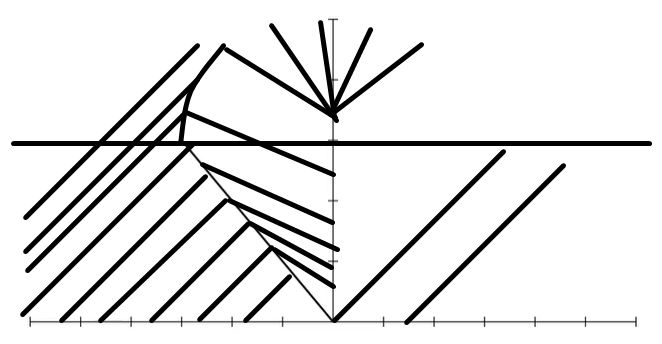
\includegraphics{Traffic Light - Turning Red}
\end{center}

\subsection{Method of Characteristics}

We will look at agns? of the form:
%
\begin{align}
  a(x, t) u_x + b(x, t) u_t + c(x, t) u & = 0\\
  u(x, 0) & = f(x)
\end{align}

Let:
%
\begin{itemize}
  \item $x(t)$ : Moving observer <- Location of observer
  \item $u(x, t)$ : function of $x$ and $t$
\end{itemize}

How does $u$ change from the observer's perspective?

How does a point in front of one move?

Find $\frac{du}{dt}$:
%
\begin{align}
  \frac{du(x(t), t)}{dt} & = \frac{du}{dt} + \frac{\p u}{\p x} \frac{dx}{dt}\\
  & = u_t + u_x \frac{dx}{dt}
\end{align}

\ex Transport Equation
%
\begin{align}
  u_t + cu_x & = 0\\
  \frac{dx}{dt} & = c\\
  \frac{du}{dt} & = 0
\end{align}

The observer is moving at speed $c$ and $u$ is not changing.

Let us consider the following:
%
\begin{align}
  u(x, 0) & = f(x)\\
  x(0) & = x_0\\
  u(0) & = u_0
\end{align}

Now, let us consider:
%
\begin{align}
  \frac{du}{dt} & = u_t + \frac{dx}{dt} u_x
\end{align}
\begin{align}
  \frac{dx}{dt} & = c\\
  x & = ct + k\\
  x & = ct + x_0\\
\end{align}
\begin{align}
  \frac{du}{dt} & = 0\\
  u & = u_0\\ & = u(x_0, 0)\\ & = f(x_0)\\ & = f(x - ct)
\end{align}

\note
%
\begin{align}
  u_t + cu_x & = 0\\
  \left< 1, c \right> \cdot \left< u_t, u_x \right> & = 0\\
  \left< 1, c \right> \cdot \left< \grad \right> & = 0
\end{align}

Here, we found the directional derivative.

\ex $u_t + cu_x = 1$ and $u(x, 0) = \sin x$
%
\begin{align}
  \frac{dx}{dt} = c & \Rightarrow x = ct + x_0\\
  \frac{du}{dt} = 1 & \Rightarrow u = t + B\\
  u(x_0, t) & = u_0\\
  & = t + u_0 = t + u(x_0, 0)\\
  & = t + \sin x_0\\
  & = t + \sin(x - ct)
\end{align}

\ex $u_t + cu_x + au = 0$, $u(x, 0) = f(x)$
%
\begin{align}
  u_t + cu_x & = -au\\
  \left< 1, c \right> \cdot \left< u_t, u_x \right> & = -au
\end{align}

If $a > 0$, directional derivative $= -au \Rightarrow$ decay
%
\begin{align}
  \frac{dx}{dt} = c & \Rightarrow x = ct + x_0
\end{align}

The following is an exponential decay (Refer to Differential Equation):
%
\begin{align}
  \frac{du}{dt} & = -au\\
  u & = De^{-at} = u_0 e^{-at}
\end{align}

When we plug in $t = 0$, we should get $f(x)$:
%
\begin{align}
  u & = f(x_0) e^{-at}\\
  & = f(x - ct) e^{-at}
\end{align}

\ex $u_t + xu_x = 0$, $u(x, 0) = f(x)$
%
\begin{align}
  \frac{dx}{dt} = x & \Rightarrow x = x_0 e^t\\
  \frac{du}{dt} = 0 & \Rightarrow u = u_0 = f(x_0) = \left(\frac{x}{e^t}\right) = f(xe^{-t})
\end{align}

\end{document}
